%%% template.tex
%%%
%%% This LaTeX source document can be used as the basis for your technical
%%% paper or abstract. Intentionally stripped of annotation, the parameters
%%% and commands should be adjusted for your particular paper - title, 
%%% author, article DOI, etc.
%%% The accompanying ``template.annotated.tex'' provides copious annotation
%%% for the commands and parameters found in the source document. (The code
%%% is identical in ``template.tex'' and ``template.annotated.tex.'')

\documentclass[conference]{acmsiggraph}

\usepackage{authblk}

\TOGonlineid{45678}
\TOGvolume{0}
\TOGnumber{0}
\TOGarticleDOI{1111111.2222222}
\TOGprojectURL{}
\TOGvideoURL{}
\TOGdataURL{}
\TOGcodeURL{}



\title{Performance Driven Redundancy Optimization of Data Layouts for Walkthrough Applications}

\author[1]{Zachary DeStefano\thanks{zdestefa@uci.edu}}
\author[1]{Shan Jiang\thanks{sjiang1714@gmail.com}}
\author[1]{Gopi Meenakshisundaram\thanks{gopi.meenakshisundaram@gmail.com}}
\author[2]{Sung-Eui Yoon\thanks{toinsert}}
\pdfauthor{Zachary DeStefano,Shan Jiang,Gopi Meenakshisundaram,Sung-Eui Yoon}
\affil[1]{University of California, Irvine}
\affil[2]{KAIST}

\keywords{Data Layout Problem, Out-Of-Core Rendering, Cache Oblivious Mesh Layout, Redundant Data Layout, Walkthrough Application}

\begin{document}

%% \teaser{
%%   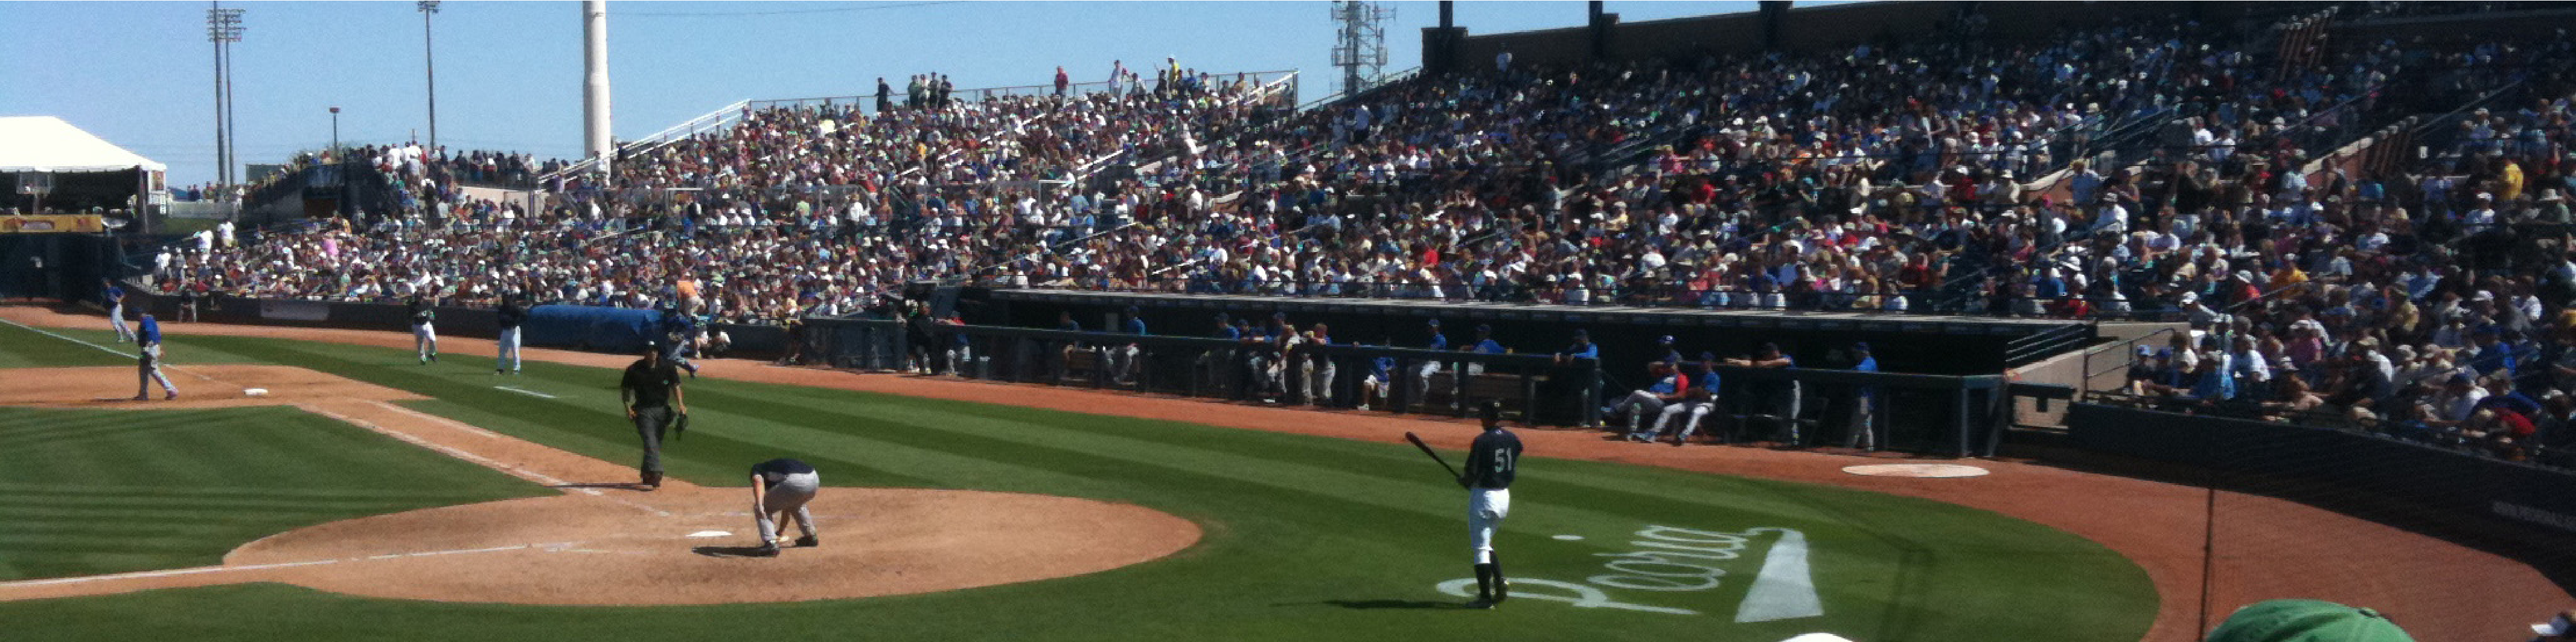
\includegraphics[height=1.5in]{images/sampleteaser}
%%   \caption{Spring Training 2009, Peoria, AZ.}
%% }

\maketitle

\begin{abstract}

Performance of interactive graphics walkthrough systems depend on the time taken to fetch the required data to render from the secondary storage to the main memory. It has been earlier established that a large fraction of this fetch time is spent on seeking the data on the hard disk. In order to reduce this seek time, redundant data storage has been proposed in the literature, but the redundancy factors of those layouts are prohibitively high.  In this paper, we develop a model for the seek time of a layout, and using this cost model, we propose an algorithm that would compute a redundant data layout with the redundancy factor that is within the user specified bounds while maximizing the performance of the system.



\end{abstract}

\begin{CRcatlist}
  \CRcat{I.3.6}{Computer Graphics}{Methodology and Techniques}{Graphics data structures and data types};
\end{CRcatlist}

\keywordlist

%% Use this only if you're preparing a technical paper to be published in the 
%% ACM 'Transactions on Graphics' journal.

\TOGlinkslist

%% Required for all content. 

\copyrightspace

\section{Introduction}


When attempting to render geometric models that contain hundreds of millions of vertices, the geometric data is too large to fit into main memory so only a small part of the model can be accessed at a given moment. When rendering a walkthrough application in this context, there is thus a seek time penalty that arises from getting data from the hard disk. This leads us to the Data Layout Problem, which is how do we lay out the data on the hard disk in such a way that minimizes the seek time required for the geometric data. Yoon et al \cite{cacheobliviouslayout} described this problem and came up with a metric to find the average seek time given the data layout as well as the access requirements of the data. An access requirement is a set of data units that will likely be accessed together during run-time.\\
\\
For the purposes of this paper, we are assuming that the relevant data units are laid out linearly on the disk. We are also assuming that the data units can be laid out in any order. Each data unit is assigned to one or more access requirements. With Yoon's definition, the average seek time ends up being the sum of the lengths of all the access requirements. We noticed that access requirements described in the paper can be very general and there could easily be data units that are far apart in the sequence but need to be accessed together. This led us to realize that if we copy data units and move them closer to other ones that share the same access requirement then we could save a lot of seek time without adding much storage space. \\
\\
We decided to formalize this idea in the form of a greedy algorithm that at each step copies the data unit which will improve seek time the most. Each step in the algorithm will copy a single data unit. We can thus stop the algorithm when we no longer have storage space to store more copies. This algorithm is thus a heuristic for the problem of given a certain amount of storage space that we are limited by, how can we minimize the seek time. 
%-----------------------

In typical walkthrough systems, data sets consisting of hundreds of millions of triangles and many gigabytes of associated data are quite common. Rendering such massive amounts of data requires out-of-core rendering algorithms that bring only the required data for rendering into main memory from secondary storage. In this process, in addition to the rendering speed, the data fetch speed also becomes critical for interactivity. Data fetch speed depends on data seek time and data transfer time. Transfer time depends only on the amount of data that is transferred. Seek time is the time taken to locate the beginning of the required data in the storage device and depends on different things depending on the storage medium. \\
\\
For a hard disk drive (HDD), this seek time depends on the speed of the disk, and the relative placement of the data units with respect to each other, also called the data layout. For a solid state drive (SSD), this seek time is usually a small constant and is independent of the location of the data with respect to each other. Because of this, \cite{ssdpaper} showed that for SSDs, cache-coherent instead of cache-oblivious data layout is enough to reduce the total data fetch time and improve cache utilization. However, SSDs have many technical problems, including limited number of data overwrites allowed, high cost, and limited capacity.  \\
\\
On the other hand, the HDD  technology (including disk technologies such as CDs, DVDs, and Blu-ray discs) has become quite reliable and inexpensive and is thus in quite widespread use. Because of this, for massive data sets hard disk drives (HDD) are still and will be the preferred medium of storage for the foreseeable future. This means that addressing the seek time bottleneck in HDDs remains critical for interactive rendering. In this paper, we leverage the inexpensive nature of HDDs to store redundant copies of data in order to reduce the seek time. 

\subsection{Main Contributions}
Redundancy based data layouts to reduce the seek time was introduced in \cite{}, in which the seek time for every access was reduced to at most one. However, in order to achieve this, the redundancy factor -- the ratio between the size of the data after introducing redundancy to the original size of the data -- was around 80 which is prohibitively high. In \cite{} the same authors related transfer volume -- which dictates the data transfer time, seek time, and redundancy and proposed a linear programming approach to optimize the data transfer and seek time in order to satisfy the total data fetch time constraint. In the process, redundancy was a hidden variable that was minimized. However, this procedure has many drawbacks: First, it provides a grouping of data units for each seek, and does not provide a data layout. It also does not relate one data group with another, and their relative layout to remove unnecessary data block duplications. Thus the redundancy minimization is not modelled after physical representation of the data layout on the disk. Second, the model for seek time is also not based on physical reality. Typically, seek time depends on the relative distance on the disk between the last data unit accessed and the current requested data unit. However, in \cite{}, seek time is simplistically modelled as  number of seeks. In other words, even if the requested data blocks are adjacent to each other, and has no separate seek time to go from one block to another, this model would count individual data blocks as one seek and add to the cost. In other words, both redundancy factor and the seek time are unrealistically modelled in \cite{}. 

In this paper, we propose a model for seek time based on the actual distance between the data blocks in the linear data layout. Using this model, and given the spatial and visual proximity of the data set for a walkthrough application, we develop an algorithm to duplicate data blocks strategically to maximize the reduction in the seek time cost while keeping the redundancy factor within the user defined bound. Note that an optimum data layout with redundancy that gives minimum seek time as well as redundancy factor is an NP-hard problem. However, we show that our greedy solution generates both the extreme cases of data layout with redundancy: a layout that has redundancy factor one (no redundancy - a simple cache oblivious layout with low number of seeks), and a layout that has exactly one disk seek for each access (with maximum redundancy factor). It also generates most of the solutions in between for varying redundancy factor constraint. 



\section{Related Work}

Massive model rendering has been a challenging field of research in computer graphics for decades. A large body of literature has been built on different aspects of solving this problem. Here we briefly discuss work in two main approaches in this topic, Out-Of-Core Rendering and Image-based Rendering. 

\subsection{Out-Of-Core Rendering}

Large-scale model rendering generally implies that the geometry data is so large that one must employ a secondary storage device during rendering. Thus, due to the nature of secondary storage devices and the architecture of modern computers, data fetching and data management for main memory can become performance bottlenecks during rendering. To remove or reduce these bottlenecks, research on out-of-core rendering aims at fetching, caching, and managing data in efficient ways. Coorea et al \cite{iwalk} introduced the iWalk system, in which octree-based spatialization is applied on geometry data, and this allowed only visible data to be retrieved from hard drives. Varadhan et al \cite{outofcore} also focused on isolating data required by each frame, but in a graph-based algorithm. A scene graph is generated in level of details and frame-to-frame visibility consistence. Parallel processing is also employed so that rendering the active part of the scene and fetching objects from the disk are done simultaneously. Sajadi et al \cite{pagebased} improved efficiency of out-of-core rendering by preprocessing the data set into a form of disk pages. The disk pages are self-contained data units with fixed size. This method avoids data management on the primitive level which reduces the time complexity by orders of magnitude. By utilizing a globally optimized data layout, caching can be further improved. Globally optimized data layout is an NP hard problem. Nevertheless, Yoon et al \cite{cacheobliviouslayout} provided a feasible method to try to compute it. Similar to other problems where an optimal permutation needs to be computed, they developed a hierarchical algorithm with a heuristic based on edge spans to get an approximated solution quickly.

\subsection{Image-Based Rendering}

Image-based rendering techniques reduce the geometry of a massive model to a view-independent mesh along with pre-rendered textures. The number of primitives to be rendered is much less than the original model. Therefore, both data transferring time and rendering time can be greatly saved. The major drawback of image-based rendering is the lack of geometry information. Zhang et al \cite{imagebasedrendering} presented a survey of image-based rendering techniques. These techniques involve sampling the space using a plenoptic function in the first stage and then rendering the continuous plenoptic function in the next stage. It is similar to the technique in signal processing of sampling a set of numbers and then using those samples to get the continuous function and reconstructing the continuous function. The paper goes into detail on various applications of these techniques. Li et al \cite{compressionimagebased} explored various compression methods for image-based rendering. Specifically, they explored the benefits of three compression algorithms. All three proved to be able to achieve real time rendering of large models and they vary in the complexity of the decoding and the compression ratio they are able to achieve. 

\subsection{Seek Time and Redundancy-based solutions}

In real time rendering, time spent on one frame can be roughly divided into data fetching time, online processing time, and rendering time. Data fetching time can be further decomposed into seek time and data transfer time. Sajadi et al \cite{ssdpaper} explored the reasons for the performance advantage of Solid-State Drives (SSD) over Hard-Disk Drives (HDD). The result shows clearly constant seek time of SSDs is the major reason that fetching data on SSDs is generally faster and more consistent than HDDs. Jiang et al \cite{singleseeklayout} minimized disk seeks to one or less for each frame by storing multiple copies of same data at different locations of secondary storage devices. These extra copies will be referred to as redundancy. The paper successfully showed that limited seeks lead to improvement of performance. However, to keep number of seeks being one or less, a large amount of redundancy is necessary, which is not practical for many applications. Jiang et al \cite{optimizingredundancy} generalized this approach by relaxing the number of seeks to a small threshold. This threshold is determined by time budget of each frame. In this way, the number of seeks required is relaxed to minimize amount of redundancy. This optimization is done through integer linear programming. This approach ended up reducing the amount of redundancy significantly. The algorithm however does not take data layout into account. It also does not take into account copies of the data that are not used and it does not take into account actual distances between these data units. For these reasons, it is not an optimal solution to our problem. 

\section{Greedy Redundancy-based Cache Oblivious Mesh Layout Algorithm}

We can formulate this problem in the following way given Yoon's metric. We are given a linear sequence of data units as well as one or more access requirements that each data unit is assigned. In Yoon's paper, he is only allowed to move the data units around. In this paper, we are allowed to copy data units, move them, and delete old copies of data units. Given this input and these 3 operations, we need to figure out how to minimize the sum of the lengths of the access requirements using the least amount of extra space as possible. For this paper, we assume that we are given a certain amount of space and need to figure out how much we can minimize the seek time.\\
\\
The algorithm in Yoon et al. computes a locally optimal solution without considering copying data units. Our algorithm takes over afterwards. W take a data unit and copy it to a place that will mean shortening at least one of the access requirements that is attached to it. If the new data unit shortens all the access requirements attached to it, then we delete the old data unit. \\
\\
There are important issues to consider in order to make this idea into an algorithm. First of all, we need to know which data units in each access requirement we should consider. We then need to figure out which access requirements to take care of first. We need to know where to insert the copied data unit. Once we copy a data unit and find its location, we need to consider whether its other access requirements should use the old or new copy. Finally, we need to decide when to stop the algorithm.  

\subsection{Which data unit in each access requirement}

Since we only care about the length of each access requirement and we can only copy a single data unit at one time, we will only be copying the data units that are on the endpoints of an access requirement. This will greatly reduce the search space of data units to consider for copying. \\
\\
The figure below shows an example access requirement. As can be observed, if we move any of the interior units, the access requirement will stay the same length or become larger. However if we move the start or end unit, the access requirement will become shorter. 
\begin{figure}[ht]
\centering
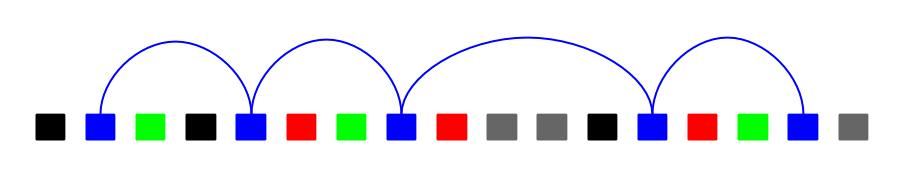
\includegraphics[width=3in]{SingleAR_start.jpg}
\caption{Data Units for a single access requirement}
\end{figure}

\subsection{Where to locate data unit}

Since we are only allowed to move one data unit at a time, in order to maximize our benefit to our current access requirement, we want to copy the start data unit to somewhere between the one after the first one and the last one. In the same manner, if the end data unit is better, we want to copy it to somewhere between the first one and the one before the last one. Below is the access requirement from the above figure with an arrow showing the locations where the start unit can be moved to. \\
\begin{figure}[ht]
\centering
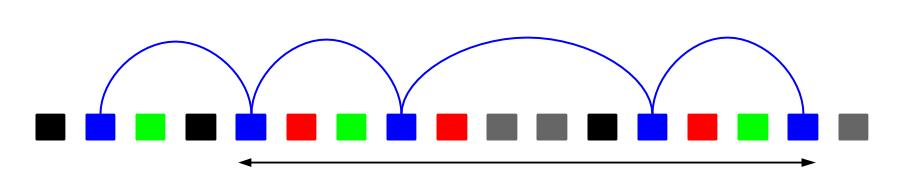
\includegraphics[width=3in]{SingleAR_afterCopy1.jpg}
\caption{Interval where the start data unit can be copied to}
\end{figure}
\\
By doing this we are guaranteed to reduce the seek time for the access requirement we care about. For our own access requirement, it won't matter where in that interval we place our data unit. However, for the other access requirements that overlap a potential place to insert our data unit, we are adding one unit of seek time. Therefore, we want to find which place will interrupt the least number of access requirements. We can assume that we have already precomputed the number of overlaps at each unit. We now have the problem of given a sequence of numbers and an arbitrary block of that sequence, what is the least number in that block. For our purposes, we will do a linear search through each entry in the block in order to find the ideal entry. While in theory there are more efficient solutions, they will be impractical for our purposes, as we will describe in the next section.

\subsection{Which data unit is used by each access requirement}

A given data unit will have a few access requirements attached to it. Thus when it is copied, it may benefit other access requirements besides the one you are currently working on. For the other access requirements, if they are shorter by using the new copy then they should do that. Otherwise, they should stick to the old copy.

\subsection{Which overall data units should be copied}

We now have established a mechanism for shortening access requirements by copying data and potentially being able to delete the old copy. We now need to figure out how to use this information to decide in what order the copying should be done. For each data unit, its total benefit is the amount that is reduces the total seek time ($EST$), which is the sum of the lengths of the access requirements. \\
\\
For a given data unit to be copied to a specified location, let $k_i$ be the benefit to access requirement $i$ that is attached to the data unit. We will say that $k_i=0$ if the access requirement will use the old copy and $k_i>0$ if the access requirement will use the new copy. Let $I$ be the set of access requirements attached to the data unit. Finally, let $M$ be the number of overlapping access requirements at the location chosen. We can now describe the benefit as follows:
\[
\Delta EST = M - \sum_{i \in I} k_i
\]
Before doing any actual copying, we will compute the above described benefit for each start and end data unit for each access requirement. We will put all the benefits into a binary search tree sorted in ascending order by benefit amount. That way we will easily be able to choose the data unit that provides the most negative change in expected seek time. We will also make a special list $L$ of cases where a data unit is copied then deleted because all the access requirements will benefit. \\
\\
Because doing the copying in $L$ does not increase the storage, we will first go through that list and do the copying. Once that list is empty we will take the data unit in the binary search tree that provides the most benefit and perform the copy. We will then recompute $L$ and the binary search tree. We will continue to do those steps until we have run out of available space for redundancy.  

\subsection{Algorithm Summary}

\begin{verbatim}

AR: access requirement

Initialize AR heap and newCopy list
for each AR P's head node and tail node U:
     Let S = next or previous node
     Set BENEFIT=distance(S,U)
     Let copy of U be U'
     Put U' in place between S and U with:
          least number of overlapping ARs
     For each AR T that also uses U
          If T will be shorter by U':
               Add T's benefit to BENEFIT
          Else:
               Add T to oldCopyList
     Add BENEFIT to heap
     If oldCopyList is empty:
          add U to newCopy list
while newCopy is not empty:
     take out random element and move the node
     Update AR heap and newCopy list
while there exists more space for redundancy:
     pop best element from heap
     copy the element U to its destination
     update affected access requirements
     update heap

\end{verbatim}

\section{Run-time and Storage Analysis}

We now need to analyze the running time and storage requirements of our algorithm. We will denote $N$ as the number of data units and $A$ as the number of access requirements. We will use $k$ as the average length of a single access requirement. The variable $Q$ will represent the number of runs of the redundancy and new copy loop. The average number of overlapping access requirements is proportional to the number of data units multiplied by the redundancy factor $r$, which is the amount of redundancy if we have a single-seek layout. Therefore, the number of overlapping access requirements is O(rN). 

\subsection{Run-time Analysis}

The Initial Construction loop is run on all A access requirements. It involves finding all the benefit information and putting it into a heap so that it is easy to figure out the best access requirement to modify first. There are log(A) operations to insert the data into the heap and a constant number of operations plus O(k) operations for the search of the AR to get the benefit information. Thus it takes a total of $O(A \cdot k \cdot logA)$ operations to do the initial construction. \\
\\
With the new copy and redundancy loops, there are O(rN) overlapping access requirements and a constant number of operations for each access requirement. Then, the algorithm reforms the heap and updates the nodes in the AR. With that, there are $O(log(A))$ operations done a constant number of times plus O(k) operations for updating the data nodes in the access requirement. Thus the redundancy and new copy loop takes $O(Q(k \cdot logA + rN))$ operations. \\
\\
This means that in total, our algorithm takes $O( k \cdot logA (Q+A) + rN)$ operations. 

\subsection{Storage Analysis}

During the run of the algorithm, we have to store the number of overlapping access requirements at each data unit, which will require $O(N)$ storage. We will also have to store a heap of access requirements, which can be stored using $O(A)$ space. We also have a list of access requirements and that information will take up $O(A)$ space. In total we thus have $O(A + N)$ storage space used during the run of the algorithm. 


\subsection{Linear search justification}

Here I justify why we do a simple linear search in the part of the algorithm where we decide where to put the new data unit. The original problem is to find the least number in an arbitrary block of a list. If $k$ is the size of the access requirement, then this gives us $O(k)$ query time. Updates will also be $O(k)$ and construction will be $O(N)$ with N being the number of data units. There are other approaches, such as a range tree or dynamic programming, that may produce better query times, but their construction and update times will be worse as well as their storage. \\
\\
With dynamic programming, we would have to maintain a matrix where an entry $(i,j)$ would contain the minimum value in that range. This would give us a $O(1)$ query time but the construction and storage would be $O(N^2)$ where N is the number of data units. The update time would be $O(N)$ when we add a data unit. Since the $N$ for this problem domain is in the hundreds of millions, that is an unacceptable storage bound. The construction run time would also be prohibitive given the magnitude of our input. \\
\\
We could use a range tree. The initial binary search tree would be sorted by index and at each entry would be a pointer to a binary search tree sorted by value. If we put the min value at each of the nodes of the initial tree, we can speed up our queries. We would get a $O(log N)$ query time, but our construction time and storage would be $O(N log N)$. Updating the data structure would take at a minimum $O(k log(N))$ time if we do careful indexing and only update the nodes that need to be updated. If we have a large access requirement, then this would represent a significant improvement in query time however given our exceptionally large input, the construction, storage, and update bounds are too prohibitive.  


\section{Theoretical Improvements over existing algorithms}

The first part of the algorithm will produce a better solution than proposed by Yoon without adding extra units. This is because our algorithm will consider cases where data units are close to each other but in different blocks of units that would be arranged in Yoon's algorithm. Consider a case where we have two access requirements of 5 data units each. Figure \ref{YoonImprovement1} shows an example of that. Figure \ref{YoonImprovement2} shows the result of using Yoon's algorithm. Because its hierarchical it would arrange the units in each block and then arrange the blocks. Thus even though the black access requirement blocks can be grouped together, Yoon's heuristic would not detect that. When our algorithm is run after Yoon's algorithm, it would find that it can shorten the black access requirements without adding redundancy so it would do that first. You would end up with the ideal solution as shown in figure \ref{YoonImprovement3}

\begin{figure}[ht]
\centering
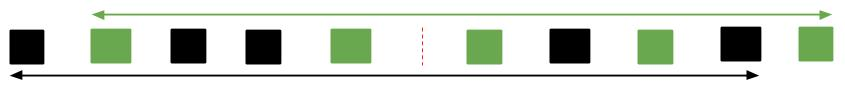
\includegraphics[width=3in]{ImprovementOverYoon_before.jpg}
\caption{Example of two access requirements of 5 data units each. The red line represents the boundary between blocks that Yoon's algorithm would use}
\label{YoonImprovement1}
\end{figure}

\begin{figure}[ht]
\centering
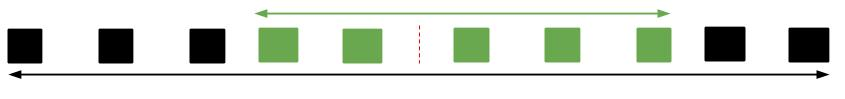
\includegraphics[width=3in]{ImprovementOverYoon_afterYoons.jpg}
\caption{The above figure after running Yoon's algorithm}
\label{YoonImprovement2}
\end{figure}

\begin{figure}[ht]
\centering
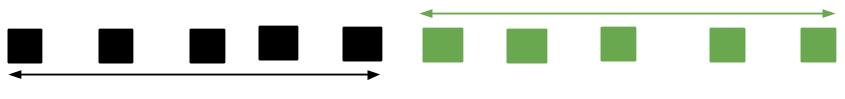
\includegraphics[width=3in]{ImprovementOverYoon_afterOurs.jpg}
\caption{The above figure after running our algorithm}
\label{YoonImprovement3}
\end{figure}

Existing algorithms for the data layout problem do not consider redundancy. Even if we find a polynomial solution to the data layout problem, we can actually achieve a seek time better than the optimal one without redundancy. Figure \ref{fig:startingProb} shows a case where that happens. The total seek time is 11 units. Without redundancy, the optimal solution is shown in Figure \ref{woRedundacy}. The seek time has been reduced to 9 units. With redundancy, the total seek time is now the minimum required which is 7 units, as shown in Figure \ref{withRedundancy}. While a reduction from 9 to 7 units may not seem dramatic, when this result is scaled up to the hundreds of millions, this makes a big difference in seek time, which we saw in practice as described in the next section.\\

\begin{figure}[ht]
\centering
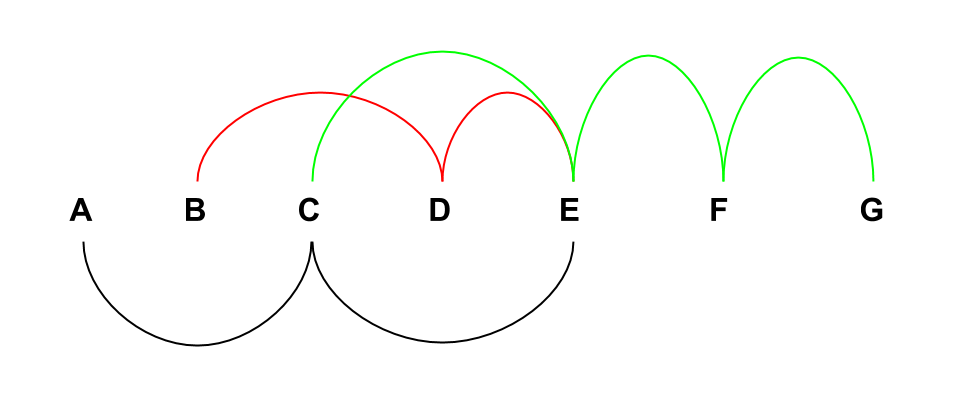
\includegraphics[width=3in]{examplePic_startingProblem.png}
\caption{Data Units with varying access requirements}
\label{fig:startingProb}
\end{figure}

\begin{figure}[ht]
\centering
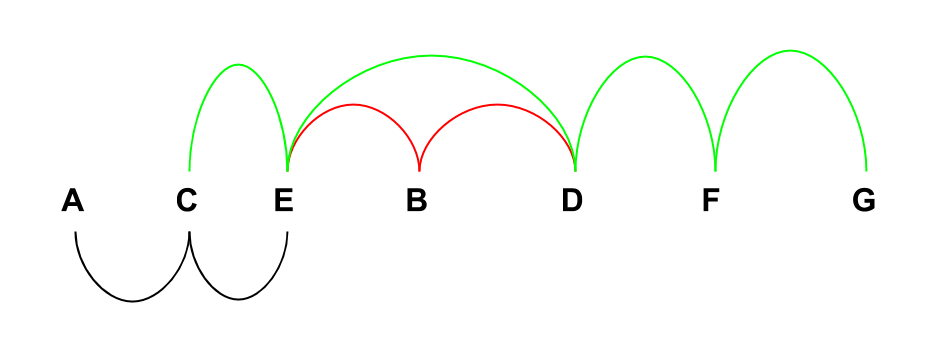
\includegraphics[width=3in]{examplePic_woRedundancy.png}
\label{woRedundacy}
\caption{Optimal layout without redundancy}
\end{figure}

\begin{figure}[ht]
\centering
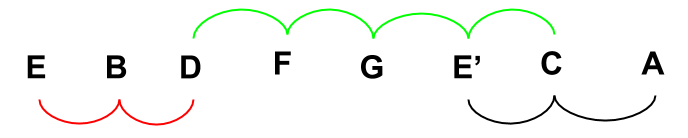
\includegraphics[width=3in]{examplePic_withRedundancy.png}
\label{withRedundancy}
\caption{Optimal layout with redundancy. The data unit E' is the redundant copy of E.}
\end{figure} 

\section{Experimental Results}

In order to implement our algorithm, we used a workstation that is a Dell T5400 PC with Intel (R) Core (TM) 2 Quad and $8GB$ main memory. The hard drive is a 1TB Seagate Barracuda with 7200 RPM and the graphics card is an nVIDIA Geforce GTX 260 with 896 MB GPU memory. The data rate of the hard drive is $120$ MB/s and the seek time is a minimum of $2$ ms per disk seek.\\
\\
Figure \ref{fig:resultall} shows the results of delays caused by fetching data on the experimental models we used. We compare the results of a cache-oblivious layout without redundancy and one with redundancy. For the layout with redundancy, we set the redundancy factor equal to 4.2. It is clear that the performance of the layout with redundancy has generally shorter delays than the cache-oblivious layout without redundancy. As can be observed from the results, although the layout with redundancy does not eliminate delays for most of sample points on the walkthrough path, it reduces delays to a small range and keeps the performance more consistent. This is the benefit we get from using our algorithm which adds redundancy. Since the algorithm tends to eliminate seeks with longer seek time first, in practice the larger delays are avoided.\\
\\

\begin{figure}[ht]
\centering
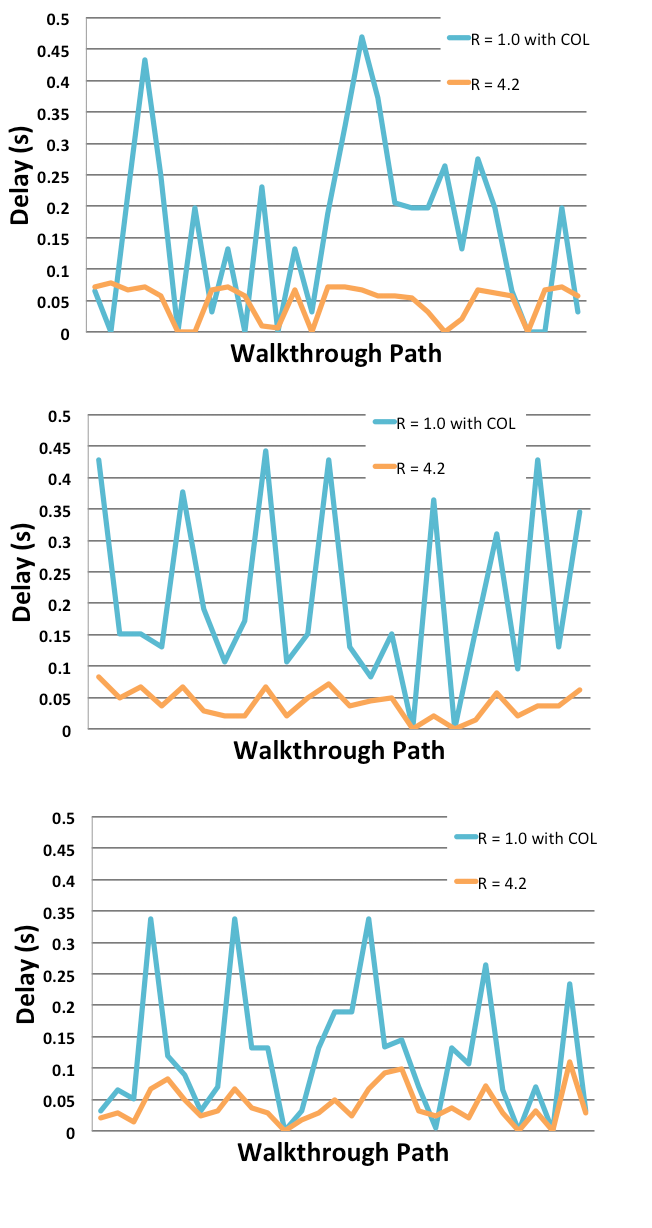
\includegraphics[width=3.0in]
{resultall.png}
  \caption{Statistics of delays caused by the fetching processes for the Sparse City model (top), the Boeing model (center), and
the Dense City model (bottom), with and without redundancy. }
  \label{fig:resultall}
\end{figure} 

\begin{figure}[ht]
\centering
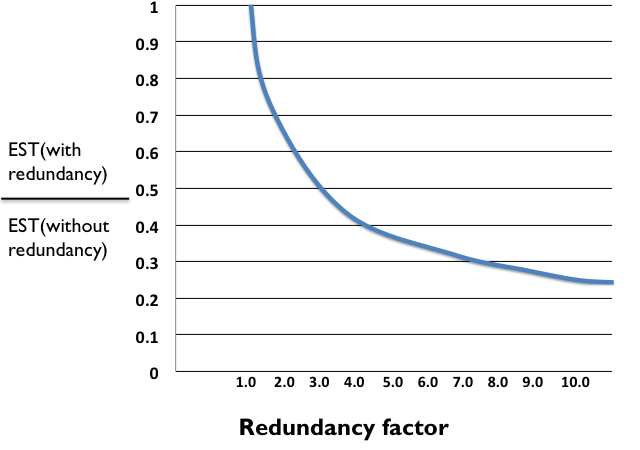
\includegraphics[width=3.0in]{statistic.png}
  \caption{Plot of the ratio of the EST of layout with redundancy over the EST of cache-oblivious mesh layout withou redundancy. }
  \label{fig:statistic}
\end{figure} 

There is another major benefit to our approach. Since each time we duplicate one data unit, we can halt it when the redundancy factor reaches a certain threshold. This helps us create a data layout with arbitrary redundancy factor without worrying about exceeding the capacity of secondary storage devices. We use this fact to test different redundancy factors and see their results. In Figure \ref{fig:statistic}, we show the results of using layouts with redundancy factors that range from 1.0 to 10.0. The y-axis in this figure is the ratio of the estimated seek time (EST) of the layout with redundancy over the EST of the layout without redundancy. This value starts at 1.0 where redundancy factor is 1.0, meaning no redundancy, and decreases as redundancy factor goes larger. We can see that the rate of this decrement is not constant, and the benefits we gain at beginning are larger than the ones we get later. This implies that most of the performance improvement resides at the earlier phase of raising redundancy factor. This implies that it is worth it to limit the redundancy factor used because after a certain point you are using much more secondary storage space without improving seek time by much. It also implies that our algorithm dramatically reduces seek time in practice by using only small redundancy factors. \\  
\\


\section{Conclusion and Future Work}

We have shown that we have an algorithm with an efficient running time and storage space for the Data Layout Problem. It achieves significant results analytically and experimentally. When walking through an extremely detailed 3D model, this algorithm can be used to ensure that the performance will not suffer. If we give the algorithm the proper access requirements with this 3D model, then the performance will be even better.\\
\\
This leads to a logical extension of this work. Since we have a good algorithm that takes over once we know the access requirements, we should figure out how to ensure there are good access requirements to begin with. One idea on how to ensure this is to check the usage history of an application and group data units together if they are accessed together with high probability. This could even be done dynamically in the sense that after a certain amount of usage and repeating on a regular basis, you recompute the optimal access requirements and then use that to recompute the optimal layout. 

\section{Acknowledgements}

To Robert, for all the bagels.

\bibliographystyle{acmsiggraph}
\bibliography{finalPaperRefs}

\end{document}
